\documentclass[journal,12pt,twocolumn]{IEEEtran}

\usepackage{setspace}
\usepackage{gensymb}
\singlespacing
\usepackage[cmex10]{amsmath}

\usepackage{amsthm}

\usepackage{mathrsfs}
\usepackage{txfonts}
\usepackage{amsmath}
\usepackage{stfloats}
\usepackage{float}
\usepackage{bm}
\usepackage{tikz}
\usepackage{pgfplots}
\pgfplotsset{compat=1.7}
\usepackage{cite}
\usepackage{cases}
\usepackage{subfig}

\usepackage{longtable}
\usepackage{multirow}

\usepackage{enumitem}
\usepackage{mathtools}
\usepackage{steinmetz}
\usepackage{tikz}
\usepackage{circuitikz}
\usepackage{verbatim}
\usepackage{tfrupee}
\usepackage[breaklinks=true]{hyperref}
\usepackage{graphicx}
\usepackage{tkz-euclide}

\usetikzlibrary{calc,math}
\usetikzlibrary{shapes.geometric, arrows}
\usepackage{listings}
    \usepackage{color}                                            %%
    \usepackage{array}                                            %%
    \usepackage{longtable}                                        %%
    \usepackage{calc}                                             %%
    \usepackage{multirow}                                         %%
    \usepackage{hhline}                                           %%
    \usepackage{ifthen}                                           %%
    \usepackage{lscape}
\usepackage{multicol}
\usepackage{chngcntr}
\usepackage{hyperref}
\hypersetup{
    colorlinks=true,
    linkcolor=blue,
    filecolor=blue,
    urlcolor=blue,
}
\DeclareMathOperator*{\Res}{Res}
\DeclareMathOperator{\sinc}{sinc}
\DeclareMathOperator{\Sa}{Sa}
\DeclareMathOperator{\rect}{rect}

\renewcommand\thesection{\arabic{section}}
\renewcommand\thesubsection{\thesection.\arabic{subsection}}
\renewcommand\thesubsubsection{\thesubsection.\arabic{subsubsection}}



\hyphenation{optical networks semiconduc-tor}
\def\inputGnumericTable{}                                 %%

\lstset{
%language=C,
frame=single, 
breaklines=true,
columns=fullflexible
}
\date{March 2021}

\makeatletter
\setlength{\@fptop}{0pt}
\makeatother

\begin{document}

\newtheorem{theorem}{Theorem}[section]
\newtheorem{problem}{Problem}
\newtheorem{proposition}{Proposition}[section]
\newtheorem{lemma}{Lemma}[section]
\newtheorem{corollary}[theorem]{Corollary}
\newtheorem{example}{Example}[section]
\newtheorem{definition}[problem]{Definition}

\newcommand{\BEQA}{\begin{eqnarray}}
\newcommand{\EEQA}{\end{eqnarray}}
\newcommand{\define}{\stackrel{\triangle}{=}}
\bibliographystyle{IEEEtran}
\raggedbottom
\setlength{\parindent}{0pt}
\providecommand{\mbf}{\mathbf}
\providecommand{\pr}[1]{\ensuremath{\Pr\left(#1\right)}}
\providecommand{\qfunc}[1]{\ensuremath{Q\left(#1\right)}}
\providecommand{\fn}[1]{\ensuremath{f\left({#1}\right)}}
\providecommand{\e}[1]{\ensuremath{E\left(#1\right)}}
\providecommand{\sbrak}[1]{\ensuremath{{}\left[#1\right]}}
\providecommand{\lsbrak}[1]{\ensuremath{{}\left[#1\right.}}
\providecommand{\rsbrak}[1]{\ensuremath{{}\left.#1\right]}}
\providecommand{\brak}[1]{\ensuremath{\left(#1\right)}}
\providecommand{\lbrak}[1]{\ensuremath{\left(#1\right.}}
\providecommand{\rbrak}[1]{\ensuremath{\left.#1\right)}}
\providecommand{\cbrak}[1]{\ensuremath{\left\{#1\right\}}}
\providecommand{\lcbrak}[1]{\ensuremath{\left\{#1\right.}}
\providecommand{\rcbrak}[1]{\ensuremath{\left.#1\right\}}}
\theoremstyle{remark}
\newtheorem{rem}{Remark}
\newcommand{\sgn}{\mathop{\mathrm{sgn}}}
\newcommand{\comb}[2]{{}^{#1}\mathrm{C}_{#2}}
\providecommand{\abs}[1]{\vert#1\vert}
\providecommand{\res}[1]{\Res\displaylimits_{#1}} 
\providecommand{\norm}[1]{\lVert#1\rVert}
%\providecommand{\norm}[1]{\lVert#1\rVert}
\providecommand{\mtx}[1]{\mathbf{#1}}
\providecommand{\mean}[1]{E\sbrak{ #1 }}
\providecommand{\fourier}{\overset{\mathcal{F}}{ \rightleftharpoons}}
%\providecommand{\hilbert}{\overset{\mathcal{H}}{ \rightleftharpoons}}
\providecommand{\system}{\overset{\mathcal{H}}{ \longleftrightarrow}}
	%\newcommand{\solution}[2]{\textbf{Solution:}{#1}}
\newcommand{\solution}{\noindent \textbf{Solution: }}
\newcommand{\cosec}{\,\text{cosec}\,}
\providecommand{\dec}[2]{\ensuremath{\overset{#1}{\underset{#2}{\gtrless}}}}
\newcommand{\myvec}[1]{\ensuremath{\begin{pmatrix}#1\end{pmatrix}}}
\newcommand{\mydet}[1]{\ensuremath{\begin{vmatrix}#1\end{vmatrix}}}
\numberwithin{equation}{subsection}
\makeatletter
\@addtoreset{figure}{problem}
\makeatother
\let\StandardTheFigure\thefigure
\let\vec\mathbf

\vspace{3cm}
\title{EE3900 Gate Assignment - 4}
\author{Adhvik Mani Sai Murarisetty - AI20BTECH11015}
\maketitle
\newpage
\bigskip
\renewcommand{\thetable}{\theenumi}

Download latex-tikz codes from 
%
\begin{lstlisting}
https://github.com/adhvik24/EE3900/blob/main/quiz1/main.tex
\end{lstlisting}
%
Download python codes from 
%
\begin{lstlisting}
https://github.com/adhvik24/EE3900/blob/main/quiz1/plot.py
\end{lstlisting}
\section*{Problem 2.27(System B)}
\textbf{(2.27(System B))}Three systems A, B, and C have the inputs and outputs indicated in Figure P2.27 -1. Determine whether each system could be LTI. If your answer is yes, specify whether there could
be more than one LTI system with the given input-output pair. Explain your answer. 

\begin{figure}[!htp]
    \centering
    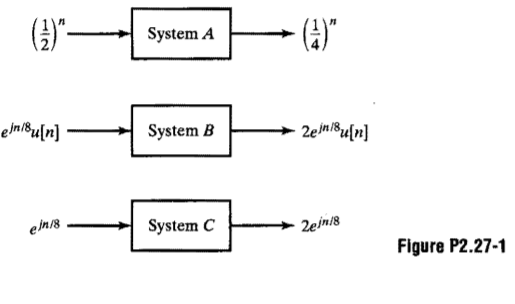
\includegraphics[width = \columnwidth]{q1.PNG}
    \caption{Systems}
    \label{f0}
\end{figure}

\section*{Solution}
\textbf{System B:}

The input signal x[n] is,
\begin{align}
    x[n]=e^{\frac{jn}{8}}u[n]\label{0}
\end{align}
The output signal y[n] is,
\begin{align}
    y[n]=2e^{\frac{jn}{8}}u[n]\label{1}
\end{align}
Then the fourier transform of x[n] is,
\begin{align}
    X\brak{e^{j\omega}}&=\sum\limits_{n=-\infty}^{n=\infty}x[n]e^{-j\omega n}\\
    &=\sum\limits_{n=-\infty}^{n=\infty}e^{\frac{jn}{8}}u[n]e^{-j\omega n}\\
    &=\sum\limits_{n=0}^{n=\infty}e^{\frac{jn}{8}}e^{-j\omega n}\\
    &=\sum\limits_{n=0}^{n=\infty}e^{-j\brak{\omega-\frac{1}{8}} n}\\
    \implies X\brak{e^{j\omega}}&=\frac{1}{1-e^{-j\brak{\omega-\frac{1}{8}}}}
\end{align}
As y[n]=2x[n],
Then the fourier transform of y[n] is,
\begin{align}
    Y\brak{e^{j\omega}}&=\frac{2}{1-e^{-j\brak{\omega-\frac{1}{8}}}}
\end{align}

Then the frequency response of the system is,
\begin{align}
    H\brak{e^{j\omega}}&=\frac{Y\brak{e^{j\omega}}}{X\brak{e^{j\omega}}}\\
    &=2
\end{align}
$\implies$ The system is a LTI system and it is unique.

\begin{figure}[!htp]
    \centering
    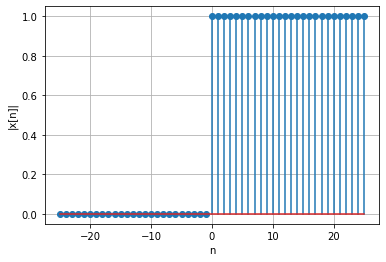
\includegraphics[width = \columnwidth]{1.PNG}
    \caption{Amplitude of x[n]}
    \label{f1}
\end{figure}

\begin{figure}[!htp]
    \centering
    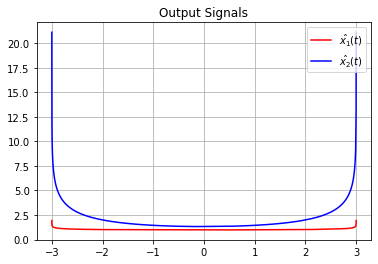
\includegraphics[width = \columnwidth]{2.PNG}
    \caption{Phase of x[n]}
    \label{f2}
\end{figure}

\begin{figure}[!htp]
    \centering
    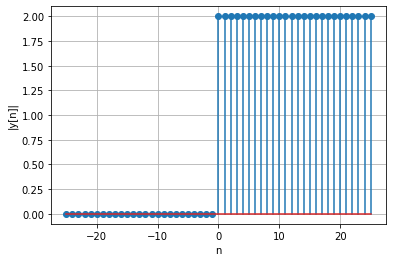
\includegraphics[width = \columnwidth]{3.PNG}
    \caption{Amplitude of y[n]}
    \label{f3}
\end{figure}

\begin{figure}[!htp]
    \centering
    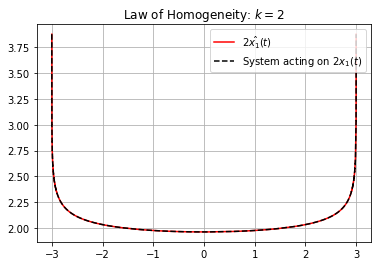
\includegraphics[width = \columnwidth]{4.PNG}
    \caption{Phase of y[n]}
    \label{f4}
\end{figure}

\end{document}
